\graphicspath{{04-KL/Figures/}}

\section{KLOE-Light Calorimeter}
\label{Sect:KL}

\subsection{Introduction}
\label{SubSect:KL_Intro}
% v2 - Domizia Orestano reviewed this (Ludovico Tortora and Mariyan Bogomilov in cc)

The KLOE-Light (KL) pre-shower sampling calorimeter is composed of extruded lead foils in which scintillating
fibres are placed in volume ratio scintillator:lead~$\sim$~2:1, ``lighter'' than the one of the KLOE experiment calorimeter~(1:1).

The fibres are 1~mm diameter BICRON BCF-12, scintillating in the blue, 1.35~mm distant from each other within a layer. The distance between two layers is 0.98~mm, one layer being shifted by half the fibre pitch with respect to the next.
Scintillation light is guided from each slab into a total of six PMTs (three on each side). Iron shields are fitted to each photomultiplier to
mitigate against large stray magnetic fields from the cooling channel (see~Fig.~\ref{fig:KL1}). The signal from each PMT is sent to a shaping amplifier (SA) module, which shapes and stretches the signal in time in order to match the sampling rate of the flash ADCs (Fig.~\ref{fig:KL2} shows the design of a single slab).
A total of 7 slabs forms the whole detector, which has an active volume of 93~cm$\times$93~cm$\times$4~cm.

With its 2.5 radiation lengths the KL is used to distinguish muons from decay electrons providing energy deposition and timing information and to act as pre-shower in front of the EMR.
The detector has been used to estimate the level of pion contamination within the MICE muon beams to be around~1\%~\cite{2016JInst..11P3001A}.
\begin{figure}
  \begin{center}
    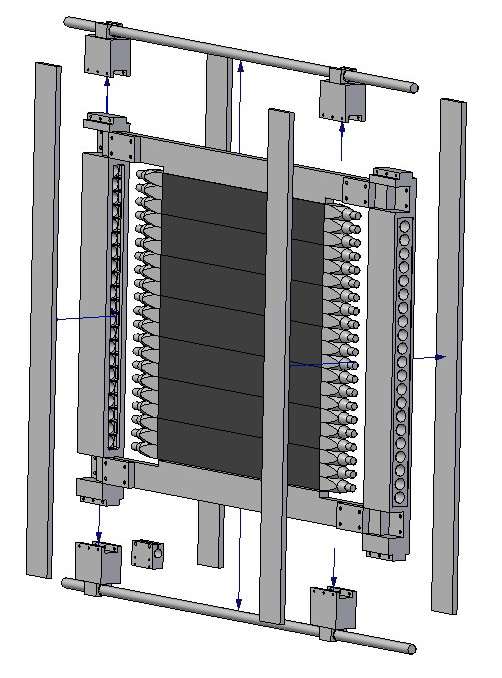
\includegraphics[width=0.4\columnwidth]{./04-KL/Figures/KL1.png}
    \caption{Magnetic shielding of KLOE-Light PMTs.}
    \label{fig:KL1}
  \end{center}
\end{figure}
\begin{figure}
  \begin{center}
    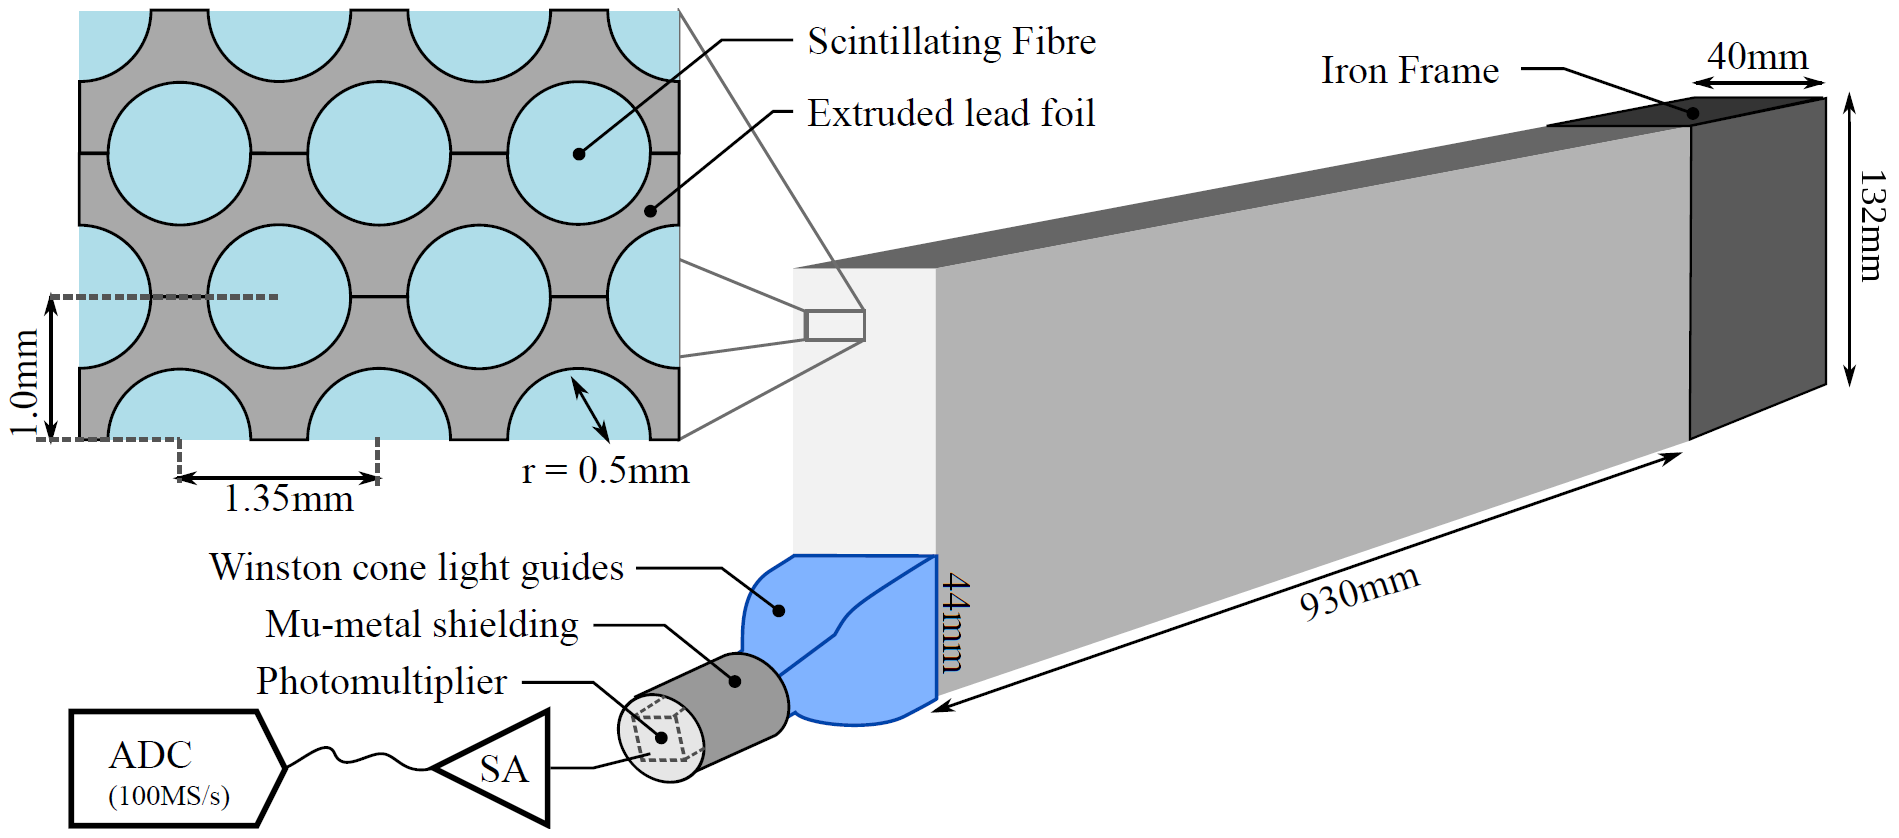
\includegraphics[width=0.8\columnwidth]{./04-KL/Figures/KL2.png}
    \caption{Single slab design of MICE KLOE-Light Calorimeter.}
    \label{fig:KL2}
  \end{center}
\end{figure}



\subsection{Performance}
\label{SubSect:KL_Performance}
